\documentclass[final]{beamer}\usepackage[]{graphicx}\usepackage[]{color}
%% maxwidth is the original width if it is less than linewidth
%% otherwise use linewidth (to make sure the graphics do not exceed the margin)
\makeatletter
\def\maxwidth{ %
  \ifdim\Gin@nat@width>\linewidth
    \linewidth
  \else
    \Gin@nat@width
  \fi
}
\makeatother

\definecolor{fgcolor}{rgb}{0.345, 0.345, 0.345}
\newcommand{\hlnum}[1]{\textcolor[rgb]{0.686,0.059,0.569}{#1}}%
\newcommand{\hlstr}[1]{\textcolor[rgb]{0.192,0.494,0.8}{#1}}%
\newcommand{\hlcom}[1]{\textcolor[rgb]{0.678,0.584,0.686}{\textit{#1}}}%
\newcommand{\hlopt}[1]{\textcolor[rgb]{0,0,0}{#1}}%
\newcommand{\hlstd}[1]{\textcolor[rgb]{0.345,0.345,0.345}{#1}}%
\newcommand{\hlkwa}[1]{\textcolor[rgb]{0.161,0.373,0.58}{\textbf{#1}}}%
\newcommand{\hlkwb}[1]{\textcolor[rgb]{0.69,0.353,0.396}{#1}}%
\newcommand{\hlkwc}[1]{\textcolor[rgb]{0.333,0.667,0.333}{#1}}%
\newcommand{\hlkwd}[1]{\textcolor[rgb]{0.737,0.353,0.396}{\textbf{#1}}}%

\usepackage{framed}
\makeatletter
\newenvironment{kframe}{%
 \def\at@end@of@kframe{}%
 \ifinner\ifhmode%
  \def\at@end@of@kframe{\end{minipage}}%
  \begin{minipage}{\columnwidth}%
 \fi\fi%
 \def\FrameCommand##1{\hskip\@totalleftmargin \hskip-\fboxsep
 \colorbox{shadecolor}{##1}\hskip-\fboxsep
     % There is no \\@totalrightmargin, so:
     \hskip-\linewidth \hskip-\@totalleftmargin \hskip\columnwidth}%
 \MakeFramed {\advance\hsize-\width
   \@totalleftmargin\z@ \linewidth\hsize
   \@setminipage}}%
 {\par\unskip\endMakeFramed%
 \at@end@of@kframe}
\makeatother

\definecolor{shadecolor}{rgb}{.97, .97, .97}
\definecolor{messagecolor}{rgb}{0, 0, 0}
\definecolor{warningcolor}{rgb}{1, 0, 1}
\definecolor{errorcolor}{rgb}{1, 0, 0}
\newenvironment{knitrout}{}{} % an empty environment to be redefined in TeX

\usepackage{alltt}
\usepackage{grffile}
\mode<presentation>{\usetheme{CambridgeUSPOL}}

\usepackage[utf8]{inputenc}
\usepackage{amsfonts}
\usepackage{amsmath}
\usepackage{natbib}
\usepackage{graphicx}
\usepackage{colortbl, xcolor}
\usepackage{array,booktabs,tabularx}
\usepackage{epstopdf}
\newcolumntype{Z}{>{\centering\arraybackslash}X}

% rysunki
\usepackage{tikz}
\usepackage{ifthen}
\usepackage{xxcolor}
\usetikzlibrary{arrows}
\usetikzlibrary[topaths]
\usetikzlibrary{decorations.pathreplacing}
%\usepackage{times}\usefonttheme{professionalfonts}  % times is obsolete
\usefonttheme[onlymath]{serif}
\boldmath
\usepackage[orientation=portrait,size=a0,scale=1.4,debug]{beamerposter}                       % e.g. for DIN-A0 poster
%\usepackage[orientation=portrait,size=a1,scale=1.4,grid,debug]{beamerposter}                  % e.g. for DIN-A1 poster, with optional grid and debug output
%\usepackage[size=custom,width=200,height=120,scale=2,debug]{beamerposter}                     % e.g. for custom size poster
%\usepackage[orientation=portrait,size=a0,scale=1.0,printer=rwth-glossy-uv.df]{beamerposter}   % e.g. for DIN-A0 poster with rwth-glossy-uv printer check
% ...
%

\usecolortheme{seagull}
\useinnertheme{rectangles}
\setbeamercolor{item projected}{bg=darkred}
% \setbeamertemplate{enumerate items}[default]
\setbeamertemplate{navigation symbols}{}
\setbeamercovered{transparent}
\setbeamercolor{block title}{fg=darkred}
\setbeamercolor{local structure}{fg=darkred}

\setbeamercolor*{enumerate item}{fg=darkred}
\setbeamercolor*{enumerate subitem}{fg=darkred}
\setbeamercolor*{enumerate subsubitem}{fg=darkred}

\setbeamercolor*{itemize item}{fg=darkred}
\setbeamercolor*{itemize subitem}{fg=darkred}
\setbeamercolor*{itemize subsubitem}{fg=darkred}

\newlength{\columnheight}
\setlength{\columnheight}{95cm}
\renewcommand{\thetable}{}
\def\andname{,}
\authornote{}

\renewcommand{\APACrefatitle}[2]{}
\renewcommand{\bibliographytypesize}{\footnotesize} 
\renewcommand{\APACrefYearMonthDay}[3]{%
{\BBOP}{#1}
{\BBCP}
}

\definecolor{maroon}{cmyk}{0,0.87,0.68,0.32}
\IfFileExists{upquote.sty}{\usepackage{upquote}}{}
\begin{document}






\date{}
\author{Micha\l{}  Burdukiewicz\inst{1}*, Piotr Sobczyk\inst{2}, Pawe\l{} Mackiewicz\inst{1}, Peter Schierack\inst{3}, Stefan R\"odiger\inst{3} \\
\small{*michalburdukiewicz@gmail.com}}

\institute{\small{\textsuperscript{1}University of Wroc\l{}aw, Department of Genomics

\vspace{0.2cm}

\textsuperscript{2}Wroc\l{}aw University of Technology, Faculty of Pure and Applied Mathematics

\vspace{0.2cm}

\textsuperscript{3}Brandenburg University of Technology Cottbus-Senftenberg, Institute of Biotechnology}

}
\title{\huge dpcR: web server and R package for analysis of dPCR experiments}

\begin{frame}
\begin{columns}
\begin{column}{.46\textwidth}
\begin{beamercolorbox}[center,wd=\textwidth]{postercolumn}
\begin{minipage}[T]{.95\textwidth}
\parbox[t][\columnheight]{\textwidth}
{


\begin{block}{Introduction}
dPCR reaction consists of multiple amplifications occurring in numerous small partitions. The result of dPCR is a binary vector describing states of partitions (positive in case of detected amplification, negative otherwise). This data is further used to estimate the main parameter, $\lambda$, which may be interpreted as the mean number of template molecules per partition.

\medskip

We created \textit{dpcR}, an open source \textbf{R} package for reproducible analysis of dPCR data, fully compatible with dMIQE requirements.
\end{block}

\vfill

\begin{block}{dpcR workflow}

\begin{figure}
\begin{center}
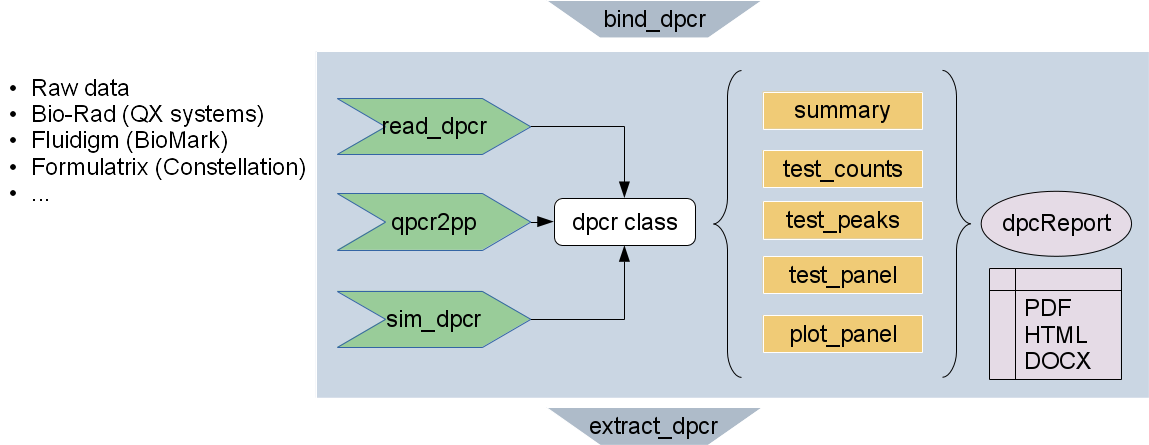
\includegraphics{dpcR_figures/dpcR_framework.png}
\end{center}
\end{figure}

The workflow diagram shows main functions available at the each step of a dPCR data analysis.

\end{block}
\vfill


\begin{block}{Data import}

Import functions limit availability of the package by determining which datasets 
can be easily processed using the provided framework. Since the RDML format for 
dPCR is not yet established, we wrote function 
\textit{read\_dpcr} streamlining data import from several systems produced by Bio-Rad, 
Fluidigm and Formulatrix. 

\smallskip

To cover experimental or not yet included systems, we 
created a ''raw data'' format (see Supplementary Files for description). The 
user can manually arrange his data in this format and import it to the 
\textit{dpcR} package. Such input files can be created in a spreadsheet program 
or a text editor.

\end{block}
\vfill

\begin{block}{Integration of qPCR data}
\begin{knitrout}
\definecolor{shadecolor}{rgb}{0.969, 0.969, 0.969}\color{fgcolor}
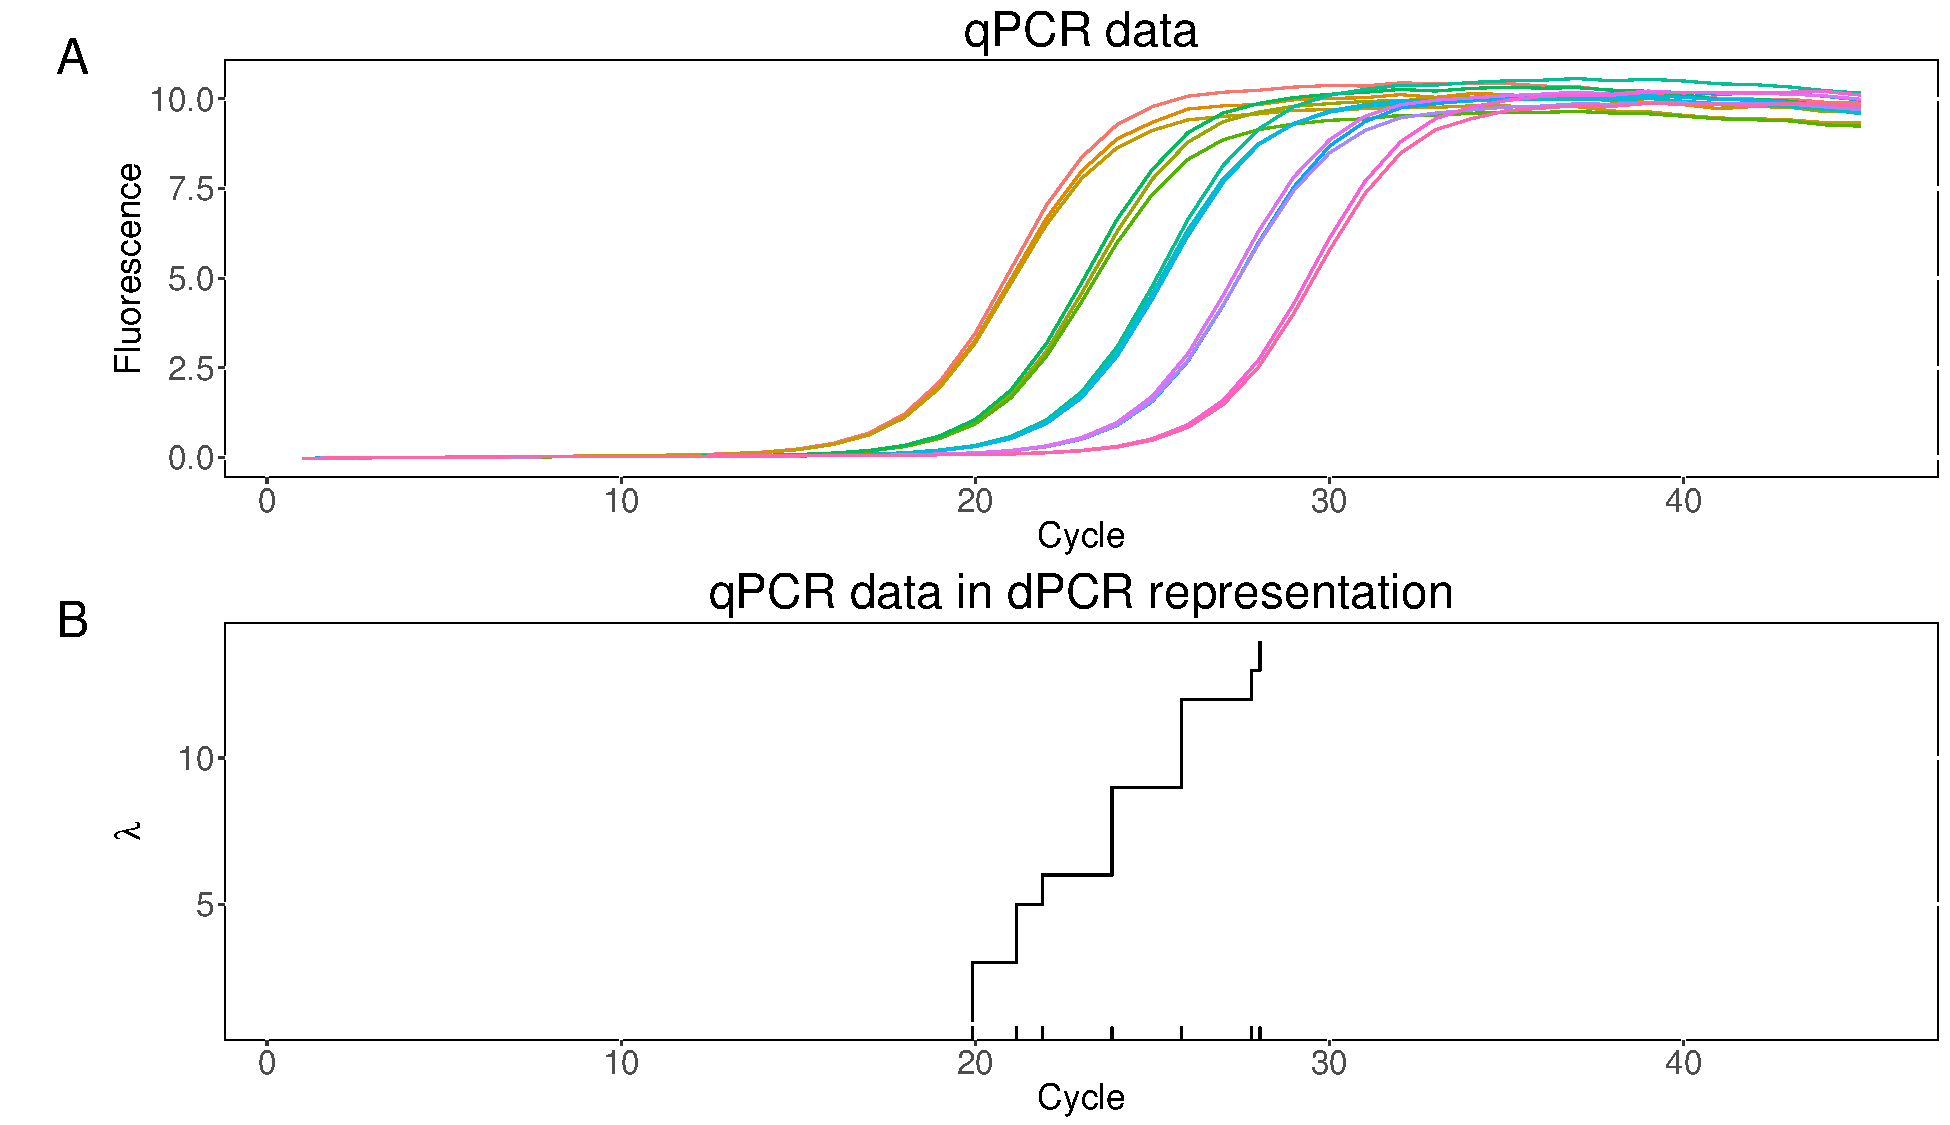
\includegraphics[width=\maxwidth]{figure/qpcr2pp-1} 

\end{knitrout}

The dPCR methodology may be used to analyze qPCR data~\citep{mojtahedi_2014}.
Quantification points (Cq) are computed using the real-time measurements of 
several amplification curves (A). Next, the Cq values are binarized and treated as 
the status of partitions effectively converting multiple qPCR experiments into a 
dPCR (B). This functionality is supported by the \textit{qpcr2pp} function.
\end{block}
\vfill

\begin{block}{Availability}
\footnotesize{
dpcReport web server: 

\url{www.smorfland.uni.wroc.pl/dpcReport}

\textit{dpcR} download:

\url{http://cran.r-project.org/package=dpcR}

}

This research was partially funded by KNOW Consortium.
\end{block}
\vfill 

\begin{block}{Bibliography}
\tiny{
\bibliographystyle{apalike}
\bibliography{dpcr}
}
\end{block}
\vfill

}
\end{minipage}
\end{beamercolorbox}
\end{column}


%new column ------------------------------------------------------    

\begin{column}{.54\textwidth}
\begin{beamercolorbox}[center,wd=\textwidth]{postercolumn}
\begin{minipage}[T]{.95\textwidth}  
\parbox[t][\columnheight]{\textwidth}
{

\begin{block}{Case study: analysis of dPCR data}

We present the functionalities of \textit{dpcR} using the previously published data set consisting of three experiments repeated twice \citep{dorazio_statistical_2015}.

% latex table generated in R 3.2.5 by xtable 1.8-2 package
% Sat May 28 10:32:59 2016
\begin{table}[ht]
\centering
\begin{tabular}{ccll}
  \toprule
Experiment & Assay & Positive partitions & Total partitions \\ 
  \midrule
CN1 & MYC & 1687 & 12765 \\ 
   \rowcolor{white}CN1 & MYC & 1787 & 13681 \\ 
  CN14 & MYC & 9913 & 13259 \\ 
   \rowcolor{white}CN14 & MYC & 11117 & 14794 \\ 
  CN16 & MYC & 13919 & 14747 \\ 
   \rowcolor{white}... & ... & ... & ... \\ 
   \bottomrule
\end{tabular}
\end{table}


\end{block}
\vfill

\begin{block}{Calculation of the uncertainty}


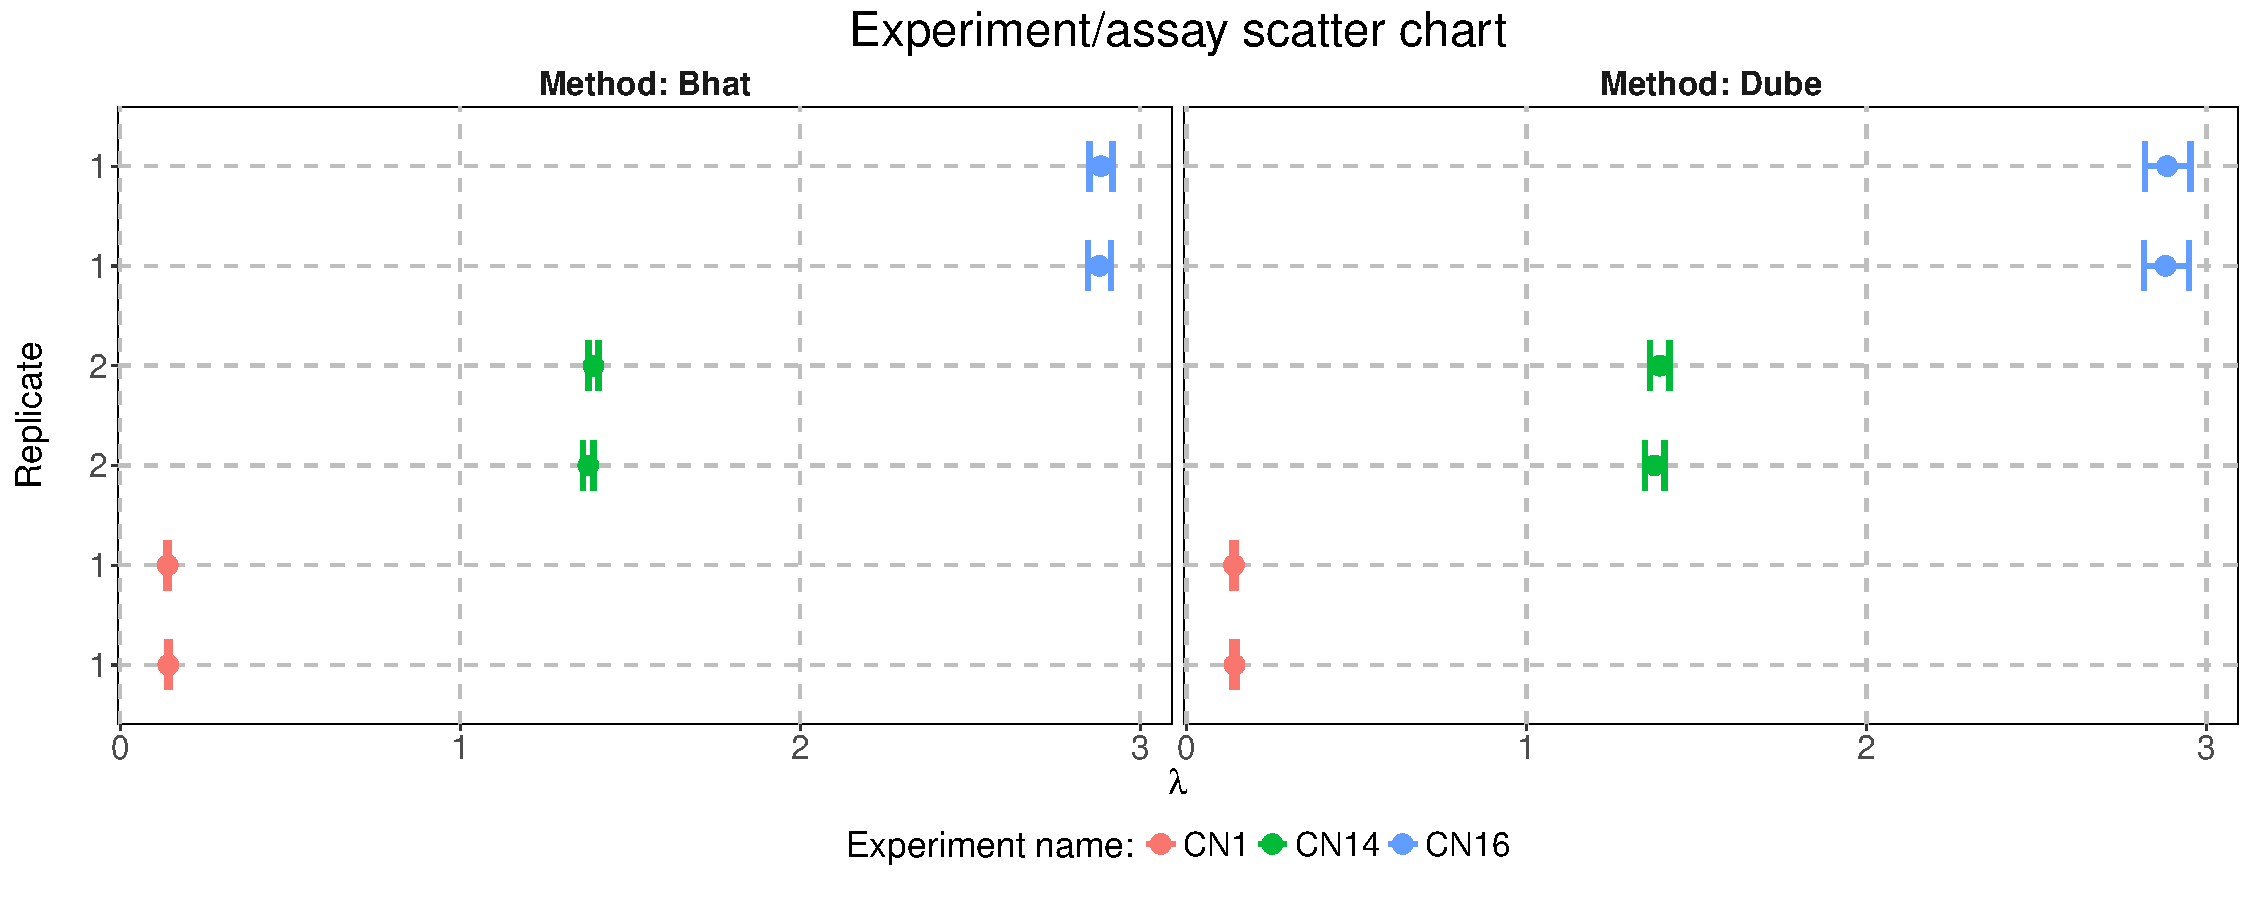
\includegraphics[width=\maxwidth]{figure/cs1-1} 


To determine the uncertainty of the estimated $\lambda$ \textit{dpcR} employs two previously 
published peer-reviewed methods \cite{dube_mathematical_2008, bhat_single_2009}.

\end{block}
\vfill

\begin{block}{Comparison of individual runs}



The \textit{dpcR} package covers peer-reviewed methods of comparing results of 
dPCR experiments. Here, by the comparison we understand a procedure, where all 
data points from all runs are considered and affect the final outcome. 


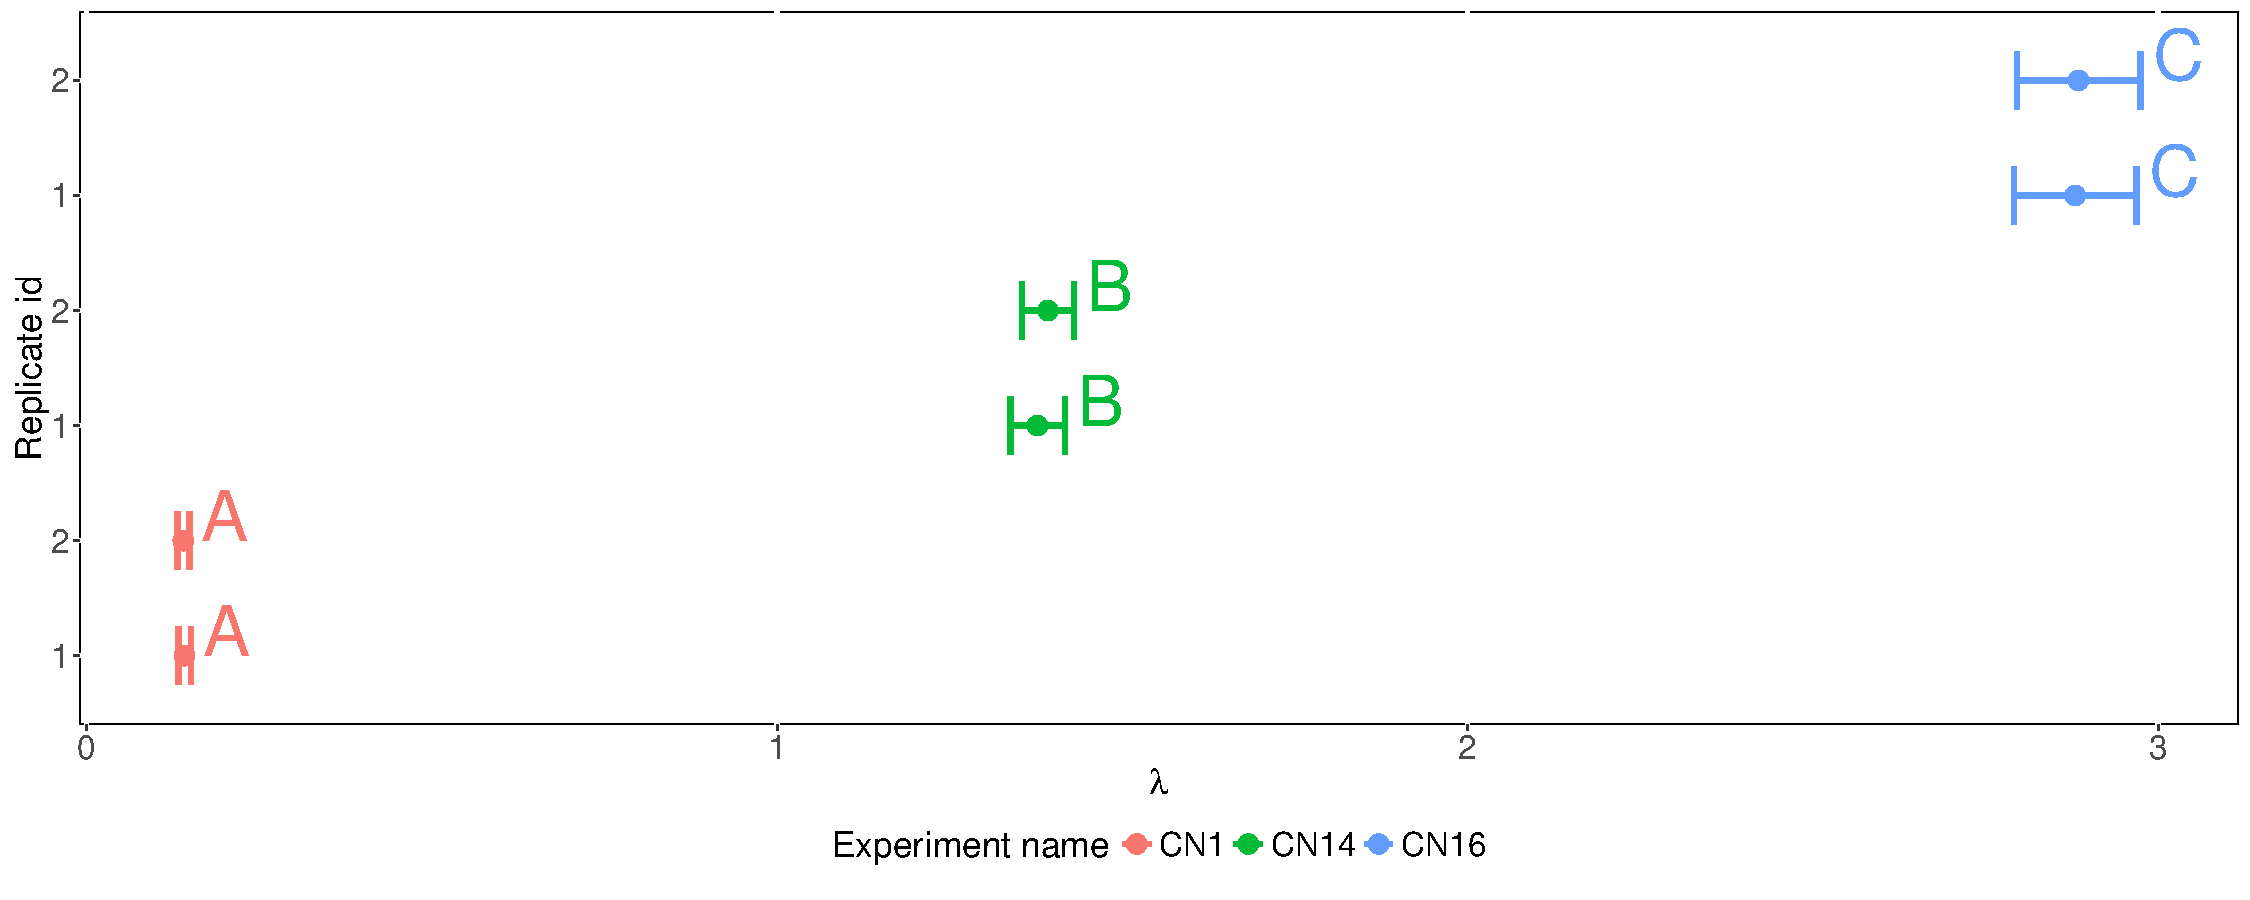
\includegraphics[width=\maxwidth]{figure/cs2-1} 


Two methods, GLM and MRT, conduct such analysis on the run level by comparing 
individual runs against each other \citep{Burdukiewicz_tba}. Additionally, we also 
implemented a method for individual dPCR experiments (not runs) 
\citep{dorazio_statistical_2015}. All methods automatically assigns experiments to
groups based on their $\lambda$ values (A, B and C on the figure above).

\end{block}
\vfill

\begin{block}{\textit{dpcReport}}

\begin{figure}
\begin{center}
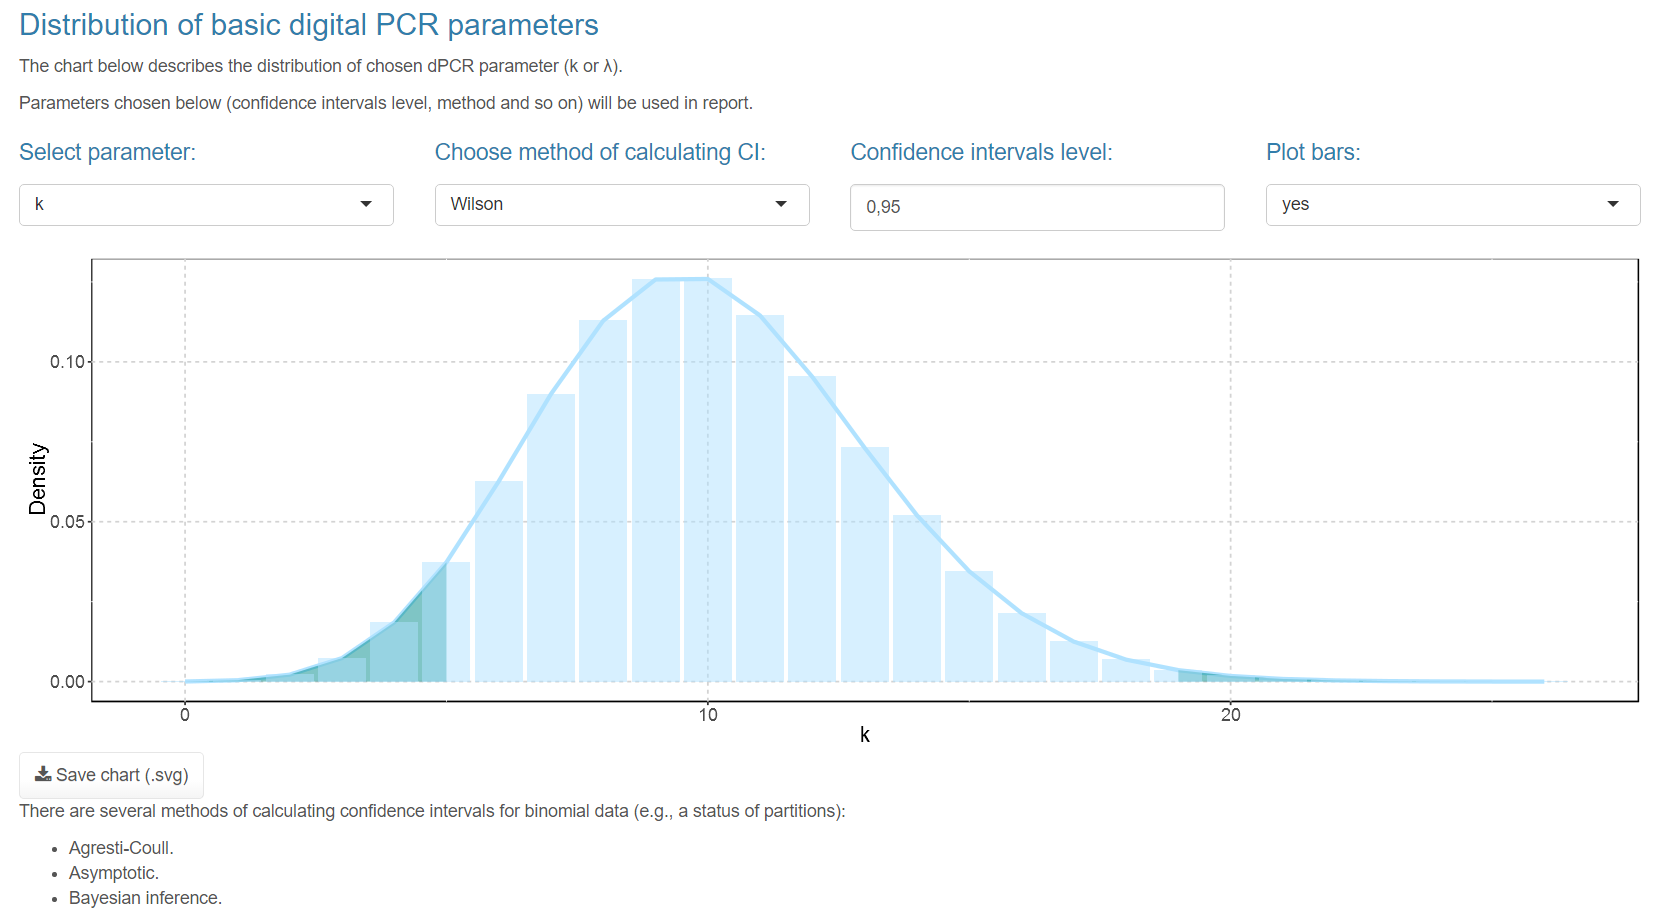
\includegraphics[width=0.76\columnwidth]{dpcR_figures/dpcReport.png}
\end{center}
\end{figure}

The majority of functions described above is also accessible using the web server \textit{dpcReport} and does not require any experience with \textbf{R}. To preserve the reproducible research principle \textit{dpcReport} generates highly customizable reports, which may even include \textbf{R} code necessary to fully recreate the analysis.

\end{block}
\vfill

\begin{block}{Funding}
\footnotesize{
This research was partially funded by KNOW Consortium, InnoProfile-Transfer 03IPT611X (BMBF) and 
KMU-innovativ-16 031B0098B (BMBF) projects.
}
\end{block}
\vfill 

}
\end{minipage}
\end{beamercolorbox}
\end{column}
\end{columns}  
\end{frame}
\end{document}
